\documentclass[11pt]{scrartcl}

\usepackage{natbib,amsmath,amsfonts}
\usepackage[utf8]{inputenc}
\usepackage[ngerman]{babel}
\usepackage{listings}
\usepackage[justification=centering]{caption}
\usepackage{subcaption}
\usepackage{pdflscape}
\usepackage{tabularx}
\usepackage{float}

%TODO: 1/25s, 1s, 1 min, 10 min, BT, WLAN jeweils mit Accel, Orien und Beides!!

\usepackage{Sweave}
\begin{document}
\Sconcordance{concordance:analyzePower.tex:analyzePower.Rnw:%
1 2 1 1 0 7 1 1 14 5 0 1 2 1 3 5 0 1 2 1 3 5 0 1 2 3 1}


\title{Die Akkulaufzeit der Samsung Gear S bei verschiedenen Arten der Datenaufzeichnung}
\author{Stefan Lüdtke}
\maketitle

\section{Einführung}
Mit der Samsung Gear S können Sensordaten, wie z.B. Beschleunigungsdaten oder Gyroskop-Daten, aufgezeichnet werden. Die Aufzeichnung sollte derart erfolgen, dass es möglichst lange dauert, bis der Akku der Uhr leer ist. Zur Aufzeichnung stehen verschiedene Verfahren zur Verfügung: 
\begin{itemize}
\item Jeder Sensorwert wird direkt in eine Datei geschrieben
\item Es werden erst einige Sensorwerte gesammelt, die dann gemeinsam in eine Datei geschrieben werden
\item Die Werte werden über Bluetooth zu einem anderen Gerät gestreamt und dort gespeichert
\item Die Werte werden über WLAN (mittels WebSocket-Protokoll) zu einem anderen Gerät gestreamt und dort gespeichert
\end{itemize}
\section{Beschreibung der Experimente}
Folgende Sensordaten wurden für die Aufzeichnung betrachtet:
\begin{itemize}
\item Beschleunigungs-Daten
\item Gyroskop-Daten
\item Beschleunigungs- und Gyroskop-Daten 
\end{itemize}
Diese wurden jeweils auf folgende Arten aufgezeichnet:
\begin{itemize}
\item jeden Sensorwert schreiben
\item Sensorwerte ein Mal pro Sekunde schreiben
\item Sensorwerte ein Mal pro Minute schreiben
\item Sensorwerte ein Mal alle 10 Minuten schreiben
\item Sensorwerte per Bluetooth streamen
\item Sensorwerte per WLAN (WebSocket-Protokoll) streamen
\end{itemize}
Für alle betrachteten Sensordaten und Aufzeichnungsarten wurde jeweils ein Experiment durchgeführt, sodass sich insgesamt 18 Experimente ergeben. Für jedes dieser Experimente wurde der Akku der Smartwatch zunächst voll geladen, dann wurden die Daten für 5 bis 9 Stunden aufgezeichnet. Zusätzlich wurde jeweils der Akkustand aufgezeichnet. Mit diesen Daten wurde dann eine lineare Regression durchgeführt, um den Zeitpunkt zu extrapolieren, zu dem die Uhr den Akkustand 0 erreicht hätte. Ein Beispiel für eine solche lineare Regression ist in Abbildung \ref{fig:linreg} zu sehen.

\begin{figure}[H]
\centering
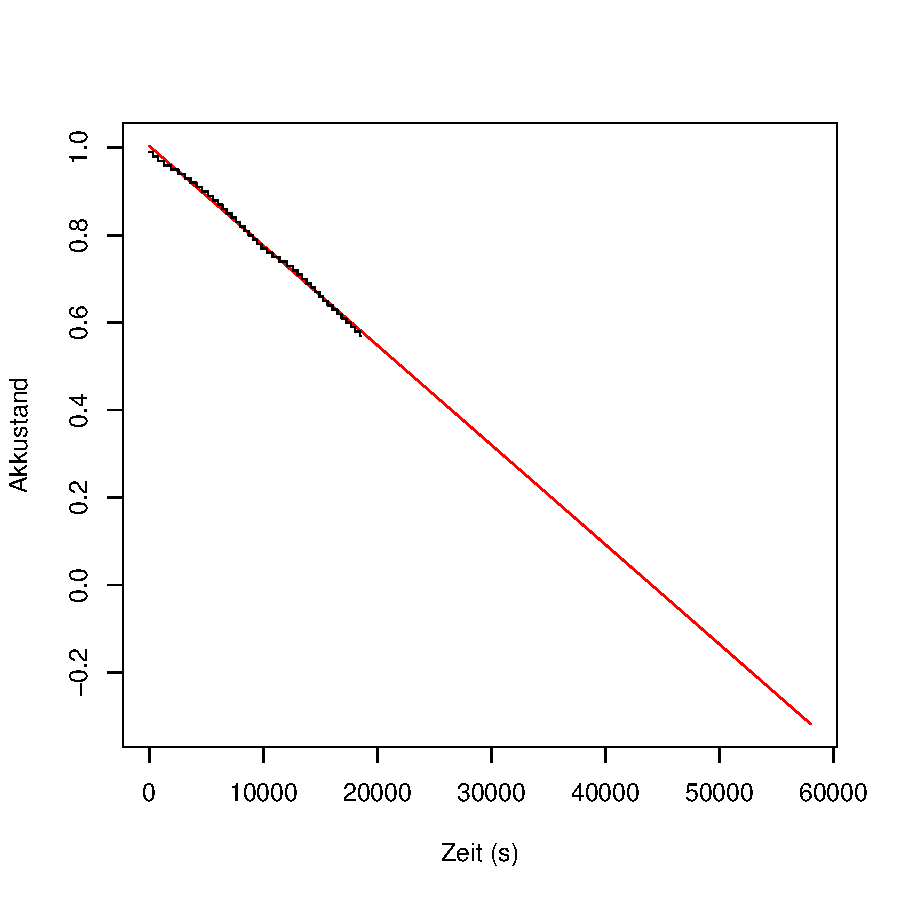
\includegraphics{analyzePower-001}
\caption{lineares Modell (rot) des Akkustandes, für das Experiment, in dem Beschleunigungsdaten 1x pro Sekunde gespeichert wurden}
\label{fig:linreg}
\end{figure}










\section{Ergebnisse}
Die Ergebnisse sind in Abbildung \ref{fig:results} dargestellt. 

\begin{figure}[H]
\centering
\includegraphics{analyzePower-006}
\caption{Noch mal zur Uebersicht}
\label{fig:results}
\end{figure}

\end{document}
